% ===========================================================================
%  06 — 评估
%
%  Verified claims: C-VLM-04, C-VLM-05, C-VLM-06, C-VLM-03b, C-VLM-07,
%                   C-DATA-01, C-VLM-03a, C-TRAIN-01
%  Likely claims:   C-VLM-03b, C-RUNTIME-01
%  Pilot claims:    descriptive/formative only (n=9), no inferential claims
% ===========================================================================
\chapter{评估}\label{ch:evaluation}

本章通过三条证据线对论文进行评估，每条证据线的声明力度各不相同。VLM 基准测试线通过在独立保留的截图上的结构化视觉事实提取度量来回答 RQ2。回放与 Harness 线通过检查基于证据的帮助循环是否可复现、可验证且可被回归夹具约束来回答 RQ1。VR 试点线通过九次参与者试验的描述性观察来回答 RQ3。这三条证据线故意不可互换：组件准确率不是学习效果，回归覆盖不是人类被试结果，试点是形成性的而非推断性的。

图~\ref{fig:evaluation-dataflow} 给出了章节级的证据映射图。它展示了基准测试产物、回放/Harness 日志和试点导出数据如何进入评估，而非将它们合并为单一类型的证明。

\begin{figure}[htbp]
  \centering
  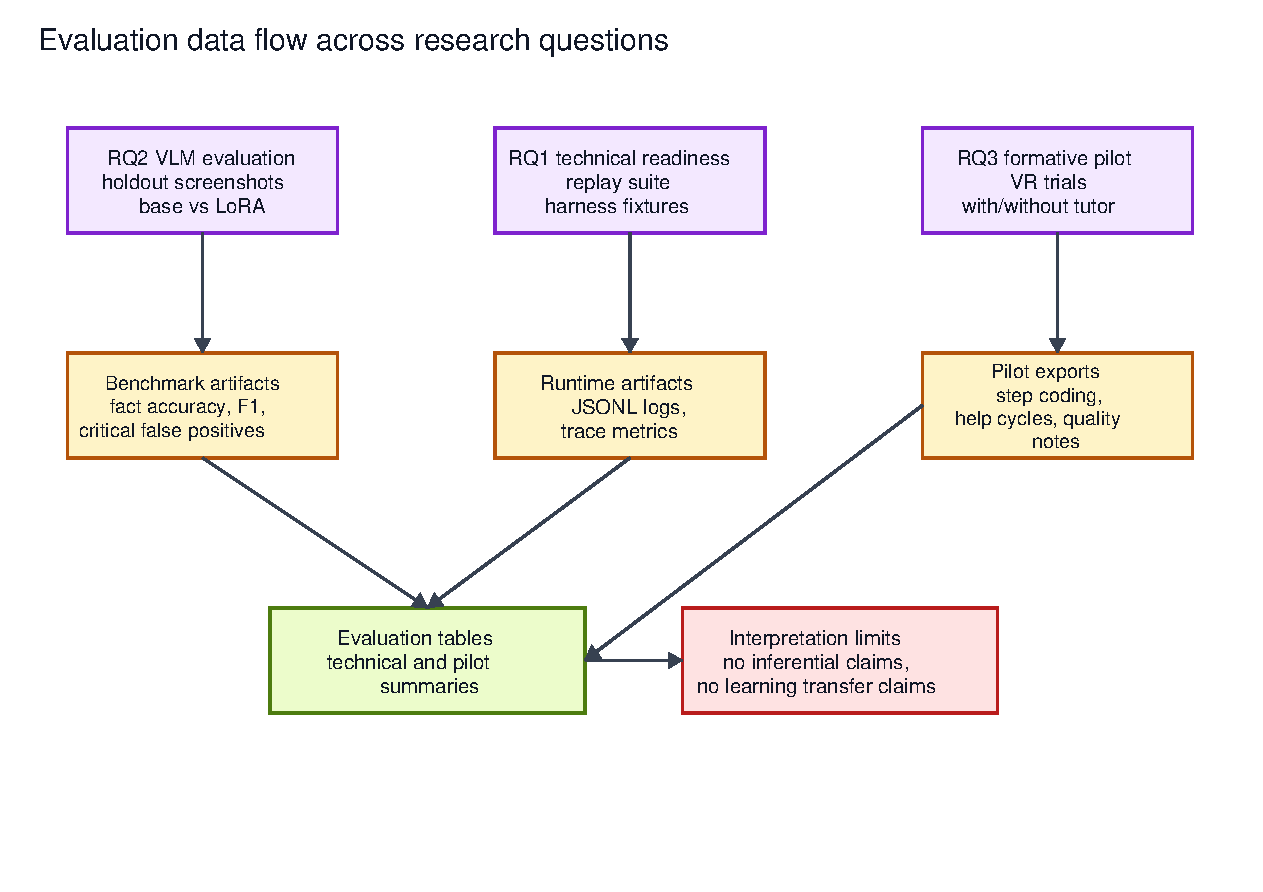
\includegraphics[width=\textwidth]{figures/fig_evaluation_dataflow.pdf}
  \caption{跨研究问题的评估与数据流。VLM 基准测试产物支撑 RQ2，回放和 Harness 日志支撑 RQ1 技术就绪性，VR 试点导出数据支撑描述性 RQ3 发现。}
  \label{fig:evaluation-dataflow}
\end{figure}

% ===========================================================================
% --- RQ2: VLM Technical Evaluation ---
% ===========================================================================
\section{RQ2：VLM 技术评估}\label{sec:eval-rq2}

技术评估关注的是：小数据 LoRA 适配能否使 VLM 在导师系统所需的狭窄任务上——从 F/A-18C 座舱显示屏截图中提取结构化视觉事实——足够可靠。模型本身不作为导师来评估，也不被认为具有程序推理能力。它被评估为一个感知组件，其输出成为帮助循环中的证据源之一。所有指标均由第~\ref{sec:method-benchmark}节描述的自动化基准测试 Harness 计算。

% ---------------------------------------------------------------------------
\subsection{数据集与训练概览}\label{sec:eval-data}

视觉事实提取任务经历了两个代际的事实本体演变。第一代（v1）定义了 8 个视觉事实并建立了初始训练流水线。第二代（v2）将本体扩展为 13 个事实，与运行时契约对齐。表~\ref{tab:dataset-summary} 总结了六个标注数据集。

\begin{table}[htbp]
\centering
\caption{标注视觉事实数据集概览。}\label{tab:dataset-summary}
\small
\begin{tabular}{@{}l c c c c l@{}}
\toprule
\textbf{数据源} & \textbf{Run} & \textbf{事实数} & \textbf{任务数} & \textbf{双语} & \textbf{用途} \\
\midrule
v1 train             & Run-001 & 8  & 180 & yes & 初始训练 \\
v1 holdout           & Run-002 & 8  & 50  & no  & 首次保留 \\
v2 newfacts holdout  & Run-002 & 13 & 50  & no  & 运行时对齐保留 \\
v2 train             & Run-003 & 13 & 220 & yes & 主要训练源 \\
v2 rebalance         & Run-005 & 13 & 122 & yes & 构成再平衡 \\
v2 random holdout    & Run-004 & 13 & 100 & no  & 独立保留 \\
\bottomrule
\end{tabular}
\end{table}

v2 训练配方将 Run-003（220 个人工审查任务）与 Run-005（122 个人工审查任务，专门采集用于再平衡代表性不足的事实状态）结合，其中 Run-005 应用两次（Run-005$\times$2）。双语导出（EN + ZH）产生总计 \textbf{928 行}训练数据。两个 v2 保留集——Run-002 newfacts（50 样本）和 Run-004 random（100 样本）——均为仅英文，并经验证与训练集的并集之间\textbf{零精确重叠}。因此，基准测试在保持同一仿真器座舱和程序领域的前提下，测试了超出精确图像重用的适配能力。

% ---------------------------------------------------------------------------
\subsection{Qwen3.5 13 事实 V2 结果}\label{sec:eval-qwen-13fact}

主要技术结果是基于 Run-003 + Run-005$\times$2 训练的 Qwen3.5-9B LoRA 适配器（928 行，4 轮，学习率 $2{\times}10^{-4}$，LoRA $r=16$，$\alpha=16$）。这是最强的 RQ2 证据，因为它在两个独立的保留集上将适配后的模型与对应的基础模型进行了比较，且使用了与运行时对齐的 13 事实本体。表~\ref{tab:qwen-13fact} 报告了结果。

\begin{table}[htbp]
\centering
\caption{13 事实 v2 基准测试：Qwen3.5-9B Base vs.\ LoRA 在两个保留集上。}\label{tab:qwen-13fact}
\small
\begin{tabular}{@{}l c c c c c c@{}}
\toprule
& \multicolumn{3}{c}{\textbf{Run-002 newfacts (50)}} & \multicolumn{3}{c}{\textbf{Run-004 random (100)}} \\
\cmidrule(lr){2-4} \cmidrule(lr){5-7}
\textbf{指标} & \textbf{Base} & \textbf{LoRA} & \textbf{$\Delta$} & \textbf{Base} & \textbf{LoRA} & \textbf{$\Delta$} \\
\midrule
JSON valid       & 1.0    & 1.0    & ---  & 0.96   & 1.0    & +0.04 \\
Schema valid     & 1.0    & 1.0    & ---  & 0.96   & 1.0    & +0.04 \\
Fact accuracy    & 0.8677 & \textbf{0.9908} & +0.1231 & 0.8038 & \textbf{0.9931} & +0.1892 \\
Macro $F_1$      & 0.4513 & \textbf{0.6515} & +0.2002 & 0.4393 & \textbf{0.6100} & +0.1707 \\
Seen $F_1$       & 0.5022 & \textbf{0.9648} & +0.4626 & 0.5659 & \textbf{0.9159} & +0.3500 \\
Exact match      & 0.10   & \textbf{0.88}   & +0.78  & 0.03   & \textbf{0.92}   & +0.89 \\
Critical FP      & 11     & \textbf{4}      & $-$7   & 70     & \textbf{8}      & $-$62 \\
\bottomrule
\end{tabular}
\end{table}

适配后的模型在 Run-002 上达到 0.9908 的事实准确率，Run-004 上达到 0.9931，样本完全匹配率分别为 0.88 和 0.92。对导师系统而言，更重要的是关键误报的变化，因为一个错误的 \texttt{seen} 状态可能使后续帮助循环的决策看起来有根基，而实际上显示证据并不存在。关键误报在 Run-002 上从 11 降至 4，在 Run-004 上从 70 降至 8。基础模型在 Run-004 上的较大失败不仅仅是格式问题：它包括 4 个 Schema 无效的响应和大量稀有状态幻觉。LoRA 适配器恢复了 JSON/Schema 可靠性，并将这种幻觉模式缩减为一组较小的可解释残余错误。

LoRA 的残余关键误报集中在完成信号而非页面存在信号上。在实践中，这意味着适配后的 VLM 足够强以支撑视觉事实流水线，但不足以被视为程序完成的独立来源。这一边界与第~\ref{ch:system-design}章的架构一致：视觉事实是证据输入，而非程序决策。

% ---------------------------------------------------------------------------
\subsection{Gemma-4 与 Qwen3.6 骨干对比}\label{sec:eval-backbones}

相同的 Run-003 + Run-005$\times$2 配方也被应用于 Qwen3.6-27B 和 Gemma-4-31B。这一对比是补充性的：它检查数据与本体配方在所评估的补充骨干上是否仍然可用，而 Qwen3.5 基础模型与 LoRA 的对比线仍然是主要技术结果。表~\ref{tab:backbone-comparison} 总结了仅 LoRA 的对比。

\begin{table}[htbp]
\centering
\caption{三种骨干上的 13 事实 v2 结果（仅 LoRA 模型）。}\label{tab:backbone-comparison}
\resizebox{\textwidth}{!}{%
\begin{tabular}{@{}l c c c c c c@{}}
\toprule
& \multicolumn{3}{c}{\textbf{Run-002 newfacts (50)}} & \multicolumn{3}{c}{\textbf{Run-004 random (100)}} \\
\cmidrule(lr){2-4} \cmidrule(lr){5-7}
\textbf{指标} & \textbf{Q3.5-9B} & \textbf{Q3.6-27B} & \textbf{G-4-31B} & \textbf{Q3.5-9B} & \textbf{Q3.6-27B} & \textbf{G-4-31B} \\
\midrule
Fact accuracy    & \textbf{0.9908} & 0.9877 & 0.9492 & \textbf{0.9931} & 0.9892 & 0.9715 \\
Seen $F_1$       & \textbf{0.9648} & 0.9479 & 0.8123 & \textbf{0.9159} & 0.9147 & 0.7959 \\
Exact match      & \textbf{0.88}   & 0.86   & 0.44   & \textbf{0.92}   & 0.86   & 0.74   \\
Critical FP      & 4      & 3      & \textbf{0} & \textbf{8} & 8      & 13     \\
\bottomrule
\end{tabular}
}
\end{table}

Qwen3.6-27B 产生了接近的结果，但在主要指标上并未超越更小的 Qwen3.5 适配器。这表明，对于这一狭窄的视觉事实任务，更大的骨干并不自动弥补一个精心匹配的小数据适配配方的价值。

Gemma-4-31B 展现出不同的错误风格。在 Run-002 上，它产生了零关键误报，但其 seen 状态召回率和样本完全匹配率低于 Qwen3.5。在 Run-004 上，Gemma 适配器相较于其基础线有显著提升，但仍然记录了比 Qwen3.5 适配器更多的关键误报。因此，对比支持一个保守的结论：13 事实数据配方可以应用于所评估的补充骨干，但部署选择仍然依赖具体骨干。Qwen3.5 是这些本地基准测试中的最佳配置；Gemma 在一个保留集上更保守，但不够完整。

% ---------------------------------------------------------------------------
\subsection{错误分析}\label{sec:eval-errors}

Qwen LoRA 的错误画像也解释了为什么第~\ref{ch:methodology}章中的本体修订是重要的。粗粒度的页面存在事实近乎完美解决。细粒度状态指示器在适配后大多数可靠，但完成类信号仍然是主要的残余风险。小文本事实可用，但对立即可辨的显示状态仍然敏感。

基础模型的主要失败模式是对稀有状态的单向幻觉。在较大的 Run-004 保留集中，FCS-MC 中间结果仅出现在 100 个样本中的 7 个中，但基础模型在额外的 60 个样本中断言该状态为 \texttt{seen}。LoRA 适配器几乎完全消除了这种弥漫性幻觉模式。剩余的误差数量更少且更可诊断，这正是基于证据的教学系统所需要的错误画像类型：运行时可以推理一组已知的有界视觉事实风险，而不是将原始 VLM 文本视为不透明的权威。

% ===========================================================================
% --- RQ1: System-Level Technical Readiness ---
% ===========================================================================
\section{RQ1：系统级技术就绪性}\label{sec:eval-rq1}

RQ1 关注的是运行时能否以技术上可靠且可审计的方式整合证据源。因此，相关证据不是参与者表现，而是帮助循环决策的可复现性、已知失败模式的回归覆盖率，以及用于后续分析的导出质量。

\subsection{回放评估}

回放评估套件定义了五个测试用例：无操作、电池开启、电池与发电机关闭、FCS 复位与 BIT，以及 INS 校准（见附录~\ref{ch:appendix}，表~\ref{tab:replay-cases}）。每个用例包含 DCS-BIOS 原始捕获，并在适用时包含视觉依赖步骤的逐帧 sidecar 文件。该套件同时覆盖了仅遥测和视觉辅助的回放条件。其作用是展示录制状态可以通过与约束实时教学的同一过程包、遥测映射、UI 映射、证据策略和 Harness 契约进行驱动。

\subsection{Harness 夹具回归}

步骤 Harness（第~\ref{sec:design-harness}节）通过覆盖矩阵中的 20 个 live-fixture 回归条目进行了覆盖。每个条目重放一个特定的实时遥测快照通过帮助循环，并断言期望的结果。这些夹具覆盖了五类就绪性风险：步骤已完成后仍然推进、错误目标阻止与修复、防止过期 VLM 证据泄漏到非视觉步骤、对移动/稳定控件的等待行为，以及交互语义的保留（如鼠标滚轮控件）。这一覆盖率并不证明导师具有教学有效性；它表明已知的证据根基失败已被捕获为可复现的测试。

\subsection{实验导出基础设施}

实验导出流水线（第~\ref{sec:method-pilot}节）已在九次实时 VR 试验中得到运用，为每次试验生成了试验摘要、步骤编码、帮助循环、操作时间线、原始事件副本和质量门控报告。全部九次导出均无阻塞性质量门控错误，且记录的过程包、分类法、UI 映射和 DCS-BIOS-to-UI 哈希值在整个研究中保持一致。这支撑了 RQ1 的测量工具部分：运行时能够从真实参与者会话中产生可审计的产物。它也暴露了一个剩余的局限。一次试验 P04 在非严格模式下通过，但出现了问卷、录像、任务和提示词关联字段缺失的元数据警告。这些警告不会使下面使用的任务指标失效，但它们表明在更大规模的受控研究之前，参与者/会话元数据 Schema 应予以收紧。

% ===========================================================================
% --- RQ3: Formative VR Pilot Study ---
% ===========================================================================
\section{RQ3：形成性 VR 试点研究}\label{sec:eval-pilot}

一项小型形成性试点研究以九名参与者开展。四名参与者在 F/A-18C 冷启动任务中使用导师系统，五名在无导师辅助的情况下练习。该试点的目的是描述性的：展示运行时、叠加层指导、视觉证据路径和导出流水线在实时 VR 使用中的表现。它不是一个有统计效力的受控实验，不支持关于学习收益、工作负荷、记忆保持、迁移或任务速度的推断性声明。方法论细节见第~\ref{sec:method-pilot}节。

\subsection{参与者与试验概览}

表~\ref{tab:pilot-overview} 总结了每位参与者的条件、完成状态、人工审查的步骤完成情况、观察时长和关键交互计数。当自动重建与人工审查不一致时，该表以人工步骤编码作为权威来源。

\begin{table}[htbp]
\centering
\caption{参与者与试验概览。观察时长为从第一次遥测事件到最后一次的挂钟间隔；对未完成试验而言，它不是完成时间的度量。}\label{tab:pilot-overview}
\small
\begin{tabular}{@{}llccccccc@{}}
\toprule
\textbf{P} & \textbf{条件} & \textbf{完成} & \textbf{步骤} & \textbf{时长 (s)} & \textbf{帮助} & \textbf{VLM} & \textbf{叠加} & \textbf{降级} \\
\midrule
P01 & without\_tutor & no & 23/33 & 2015 & 0 & 0 & 0 & 0 \\
P02 & without\_tutor & no & 27/33 & 739  & 0 & 0 & 0 & 0 \\
P03 & without\_tutor & no & 24/33 & 243  & 0 & 0 & 0 & 0 \\
P06 & without\_tutor & no & 29/33 & 269  & 0 & 0 & 0 & 0 \\
P07 & without\_tutor & no & 19/33 & 218  & 0 & 0 & 0 & 0 \\
\midrule
P04 & with\_tutor    & yes & 33/33 & 442  & 19 & 6  & 22 & 6 \\
P05 & with\_tutor    & yes & 33/33 & 317  & 7  & 2  & 6  & 2 \\
P08 & with\_tutor    & yes$^*$ & 33/33 & 332  & 7  & 5  & 10 & 4 \\
P09 & with\_tutor    & yes & 33/33 & 1033 & 44 & 10 & 44 & 9 \\
\bottomrule
\end{tabular}

$^*$P08：自动摘要报告未完成；人工编码确认 33/33 完成（见下方数据质量注记）。
\end{table}

\textbf{完成情况。}所有四名有导师辅助的参与者在人工审查下达到了最终的 33 步状态。五名无导师辅助的参与者无一完成完整程序；他们在完成 19--29 步后停止。无导师辅助条件下最常见遗漏的步骤是 S18（FCS-MC BIT 页面）、S19（FCS BIT 最终 GO）和 S27（襟翼开关至 AUTO），每位步骤均被全部五名无导师辅助参与者遗漏。

\textbf{观察时长。}有导师辅助的试验范围为 317\,s 至 1033\,s（中位数 387\,s）。无导师辅助试验范围为 218\,s 至 2015\,s。这些值仅作为追踪时长报告。由于无导师辅助试验在不同的程序节点结束，这些时长不是条件间的完成时间比较。

\subsection{程序性错误}

表~\ref{tab:pilot-errors} 报告了每参与者的人工错误计数。

\begin{table}[htbp]
\centering
\caption{每参与者人工程序性错误计数（来自人工步骤编码）。OM = 遗漏，CO = 执行错误，OR = 顺序错误，PA = 提示/辅助错误，SV = 状态违反。}\label{tab:pilot-errors}
\small
\begin{tabular}{@{}llccccc@{}}
\toprule
\textbf{P} & \textbf{条件} & \textbf{OM} & \textbf{CO} & \textbf{OR} & \textbf{PA} & \textbf{SV} \\
\midrule
P01 & without\_tutor & 8  & 0 & 1 & 0 & 1 \\
P02 & without\_tutor & 0  & 0 & 0 & 1 & 0 \\
P03 & without\_tutor & 7  & 0 & 2 & 0 & 2 \\
P06 & without\_tutor & 2  & 0 & 0 & 2 & 0 \\
P07 & without\_tutor & 11 & 0 & 0 & 0 & 0 \\
\midrule
P04 & with\_tutor    & 0  & 3 & 0 & 3 & 1 \\
P05 & with\_tutor    & 0  & 3 & 0 & 3 & 0 \\
P08 & with\_tutor    & 0  & 0 & 0 & 0 & 0 \\
P09 & with\_tutor    & 0  & 3 & 0 & 2 & 0 \\
\bottomrule
\end{tabular}
\end{table}

\textbf{遗漏错误。}无导师辅助条件显示出明显的遗漏模式：五分之四的参与者记录了遗漏错误，三名参与者记录了七个或以上的遗漏。相比之下，有导师辅助条件记录了零人工遗漏错误；在人工审查下，每个必需的步骤最终都被完成。

\textbf{执行错误与提示错误。}有导师辅助条件显示出不同的错误画像。CO 和 PA 错误出现在 P04、P05 和 P09 中，而 P08 在审查后没有人工编码的程序性错误。这些错误是辅助耦合型的：参与者通常遵循了指导，但指导或其时机并未完全匹配程序规范或当前状态。这是一个重要的形成性发现。导师条件与程序中的持续推进相关联，但也引入了新的指导风险类别，这些风险应在更大规模的研究之前予以减少。

\textbf{错误总计。}无导师辅助参与者平均有 7.4 个人工错误；有导师辅助参与者平均有 4.5 个。这一差异仅为描述性，不应被解读为推断性的处理效应。更重要的是定性的发现：无导师辅助的错误以遗漏为主，而有导师辅助的错误转向执行错误、提示/辅助错误和一次状态违反。

\subsection{教学交互}

表~\ref{tab:pilot-tutor} 总结了四次有导师辅助试验的教学交互指标。

\begin{table}[htbp]
\centering
\caption{教学交互摘要（仅导师辅助条件）。}\label{tab:pilot-tutor}
\small
\begin{tabular}{@{}lccccc@{}}
\toprule
\textbf{P} & \textbf{帮助循环} & \textbf{VLM 调用} & \textbf{叠加执行} & \textbf{叠加拒绝} & \textbf{降级} \\
\midrule
P04 & 19 & 6  & 22 & 0 & 6 \\
P05 & 7  & 2  & 6  & 0 & 2 \\
P08 & 7  & 5  & 10 & 0 & 4 \\
P09 & 44 & 10 & 44 & 0 & 9 \\
\midrule
合计 & 77 & 23 & 82 & 0 & 21 \\
\bottomrule
\end{tabular}
\end{table}

全部 77 个帮助循环使用了模型生成路径；没有循环降级到仅确定性响应。四次有导师辅助试验中 VLM 调用合计 23 次。当前过程包将 S08、S15、S18 和 S19 视为视觉优先步骤，但试点日志也揭示了在非视觉或已推进状态下偶尔出现不必要的 VLM 调用。这种过度触发是运行时调优问题，而非参与者结果。

\textbf{叠加拒绝率为零}：全部 82 个已执行的叠加操作通过了运行时的证据根基、白名单和 Schema 检查。21 个降级事件（21/77 = 帮助循环的 27\%）并非仅确定性的降级。它们是 Harness 或验证器对模型提议的叠加层计划的修复，例如将粗粒度的显示目标重映射为更具体的 BIT-root 子状态目标。这支撑了 RQ1 的声明：实时系统能够在叠加层到达之前修复模型输出，同时也显示了模型在哪些地方仍然需要运行时纠正。

\subsection{数据质量注记}

\begin{enumerate}
\item \textbf{P08 自动摘要校正。}自动化流水线将 P08 报告为未完成（5/33 步）。人工遥测审查确认所有 33 步均达到所需状态。自动流水线未能从被动遥测中为视觉优先步骤重建完成证据。人工编码覆盖自动摘要；P08 报告为已完成，0 个人工错误。

\item \textbf{P02 问卷排除。}P02 的问卷 JSON 文件包含内部参与者 ID 不匹配，表明标注错误。P02 被排除在任何工作负荷、TLX 或信心摘要之外。来自试验摘要和人工步骤编码的任务指标保留。

\item \textbf{质量门控解释。}全部九次参与者导出均无阻塞性质量门控错误通过。P04 仍然存在问卷、录像、任务和提示词关联字段缺失的元数据警告。这些警告限制了问卷级分析和可追溯性，但不与表~\ref{tab:pilot-overview}和表~\ref{tab:pilot-errors}中报告的任务指标相矛盾。

\item \textbf{时长解释。}无导师辅助试验在参与者无法继续推进的不同程序节点结束。观察时长仅为完整性报告，不支持条件间的完成时间比较。

\item \textbf{非随机分配。}参与者基于排期可用性被分配到条件，非随机化。先前的 DCS 和 VR 经验在参与者之间有所不同（见附录~\ref{ch:appendix}，表~\ref{tab:pilot-participants}）。
\end{enumerate}

\subsection{试点发现总结}

本次试点提供了三项形成性证据。第一，导师条件在这些四次试验中支撑了程序推进：全部四名有导师辅助参与者完成了经审查的 33 步程序，而五名无导师辅助参与者无一完成。第二，错误模式发生了变化。导师条件消除了编码遗漏，但并未消除所有程序性问题；辅助耦合的 CO 和 PA 错误出现在四分之三的有导师辅助试验中。第三，实时教学基础设施在 77 个帮助循环和 82 个叠加层执行中无叠加拒绝地运行，同时记录了审计所需的修复和降级决策。

纵观全章，最强的实证声明是 RQ2 VLM 结果：小数据 LoRA 适配在本地保留集上产生了可靠得多的 13 事实视觉提取器。RQ1 得到了回放、Harness 和导出证据的支撑，表明运行时可以被审计和回归测试。RQ3 得到了已完成的形成性 VR 试点的支撑，但仅达到描述性强度。这些结果并未建立学习改进、工作负荷降低、技能获取加速、记忆保持或迁移。这些声明需要更大规模、随机化、受控的研究。
